\section{Experiment}

\subsection{Goals and Hypothesis}
\textbf{H1}: RubberEdge will reduce clutch invocations required to traverse a pointer to a target when compared to conventional Transfer Functions, Constant Gain and Acceleration.

\textbf{H2}: The time taken to traverse a pointer to a target using the RubberEdge Function will be less than existing Constant and Acceleration Transfer Functions.


\subsection{Apparatus}\label{section:apparatus}
The laptop used for the experiments was a Dell XPS 15 9560\cite{XPSZealand}, it featured a 15 inch display with a resolution of 3840px x 2160px, giving it 282.4 \gls{PPI}. The Windows 10 operating system, with display scaling set to 175\% for an effective resolution of 2194px x 1234px was used on the laptop.

\begin{figure}[h]
    \centering
    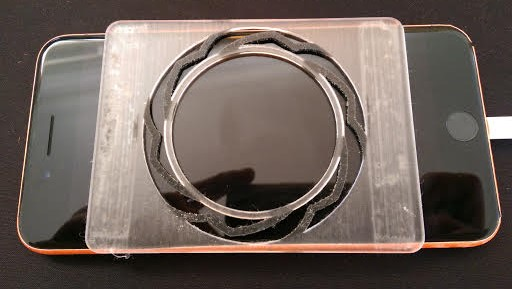
\includegraphics[width=0.9\columnwidth]{Aparatus}
    \caption{The RubberEdge device, adhered to the screen of an iPhone 7 Plus}
    \label{fig:apparatus}
\end{figure}

As discussed in Section \ref{section:interface_data} problems were encountered when getting the absolute position of a participants finger on the touchpad, due to time constraints a compromised was settled on where an iPhone 7 Plus was used, with the RubberEdge interface adhered to the screen with double sided tape, as shown in Figure \ref{fig:apparatus}. A separate web page was then created, that would be navigated to on the phone, from which touch input could be transmitted to the laptop hosting a web server over web sockets.


\subsection{Experiment Interface}
An experiment based on Fitts' law was deemed to be an adequate way of testing the conditions. The interface is based off the Visualising Fitts Law\cite{Wallner2017AnD3} web page, which follows the ISO 9241-9 standard\cite{ISODevices}

The web interface used in the experiment was built using the Polymer framework\cite{WelcomeProject}.

Participants were first presented with an instructions page outlining how the RubberEdge device is intended to be used. After completing a short pre-experiment survey, they calibrate the isotonic and elastic zones for their finger.
The calibration processed involved tracing with one finger around the edge of the inner ring of the RubberEdge device, without putting pressure on the ring. Calibration is important as participants had different sized fingers and would orient their hands differently relative to the device.

To calculate the isotonic and elastic zone a circle fitting algorithm\cite{Maisonobe2007FindingPoints} was applied which takes a set of points and finds the midpoint and radius of a circle that best represents those points. This circle defines the isotonic zone, points falling outside the circle are considered to be in the elastic zone.

From this entries in and out of the elastic zone can be tracked by measuring the distance between a given point and the centre of the defined isotonic zone.

\subsection{Task and Stimuli}
The Fitts' law task is to move the pointer in the indicated circle, upon which release the finger from the touchpad a new target would be generated. Nine targets are spaced equally around a central point, which is in the centre of the screen. Targets are selected in an opposing order, which means the user has to move the pointer and equal distance to select each target.

The distances selected based on relative pixel coordinates in the web browser were 500px, 750px, 1000px when translated to mm this works out to be 79mm, 118mm, 157mm respectively.
The selected widths were 25px, 50px, 75px and translated they are 3.9mm, 7.9mm, 11.8mm respectively.

\begin{figure}[h]
    \centering
    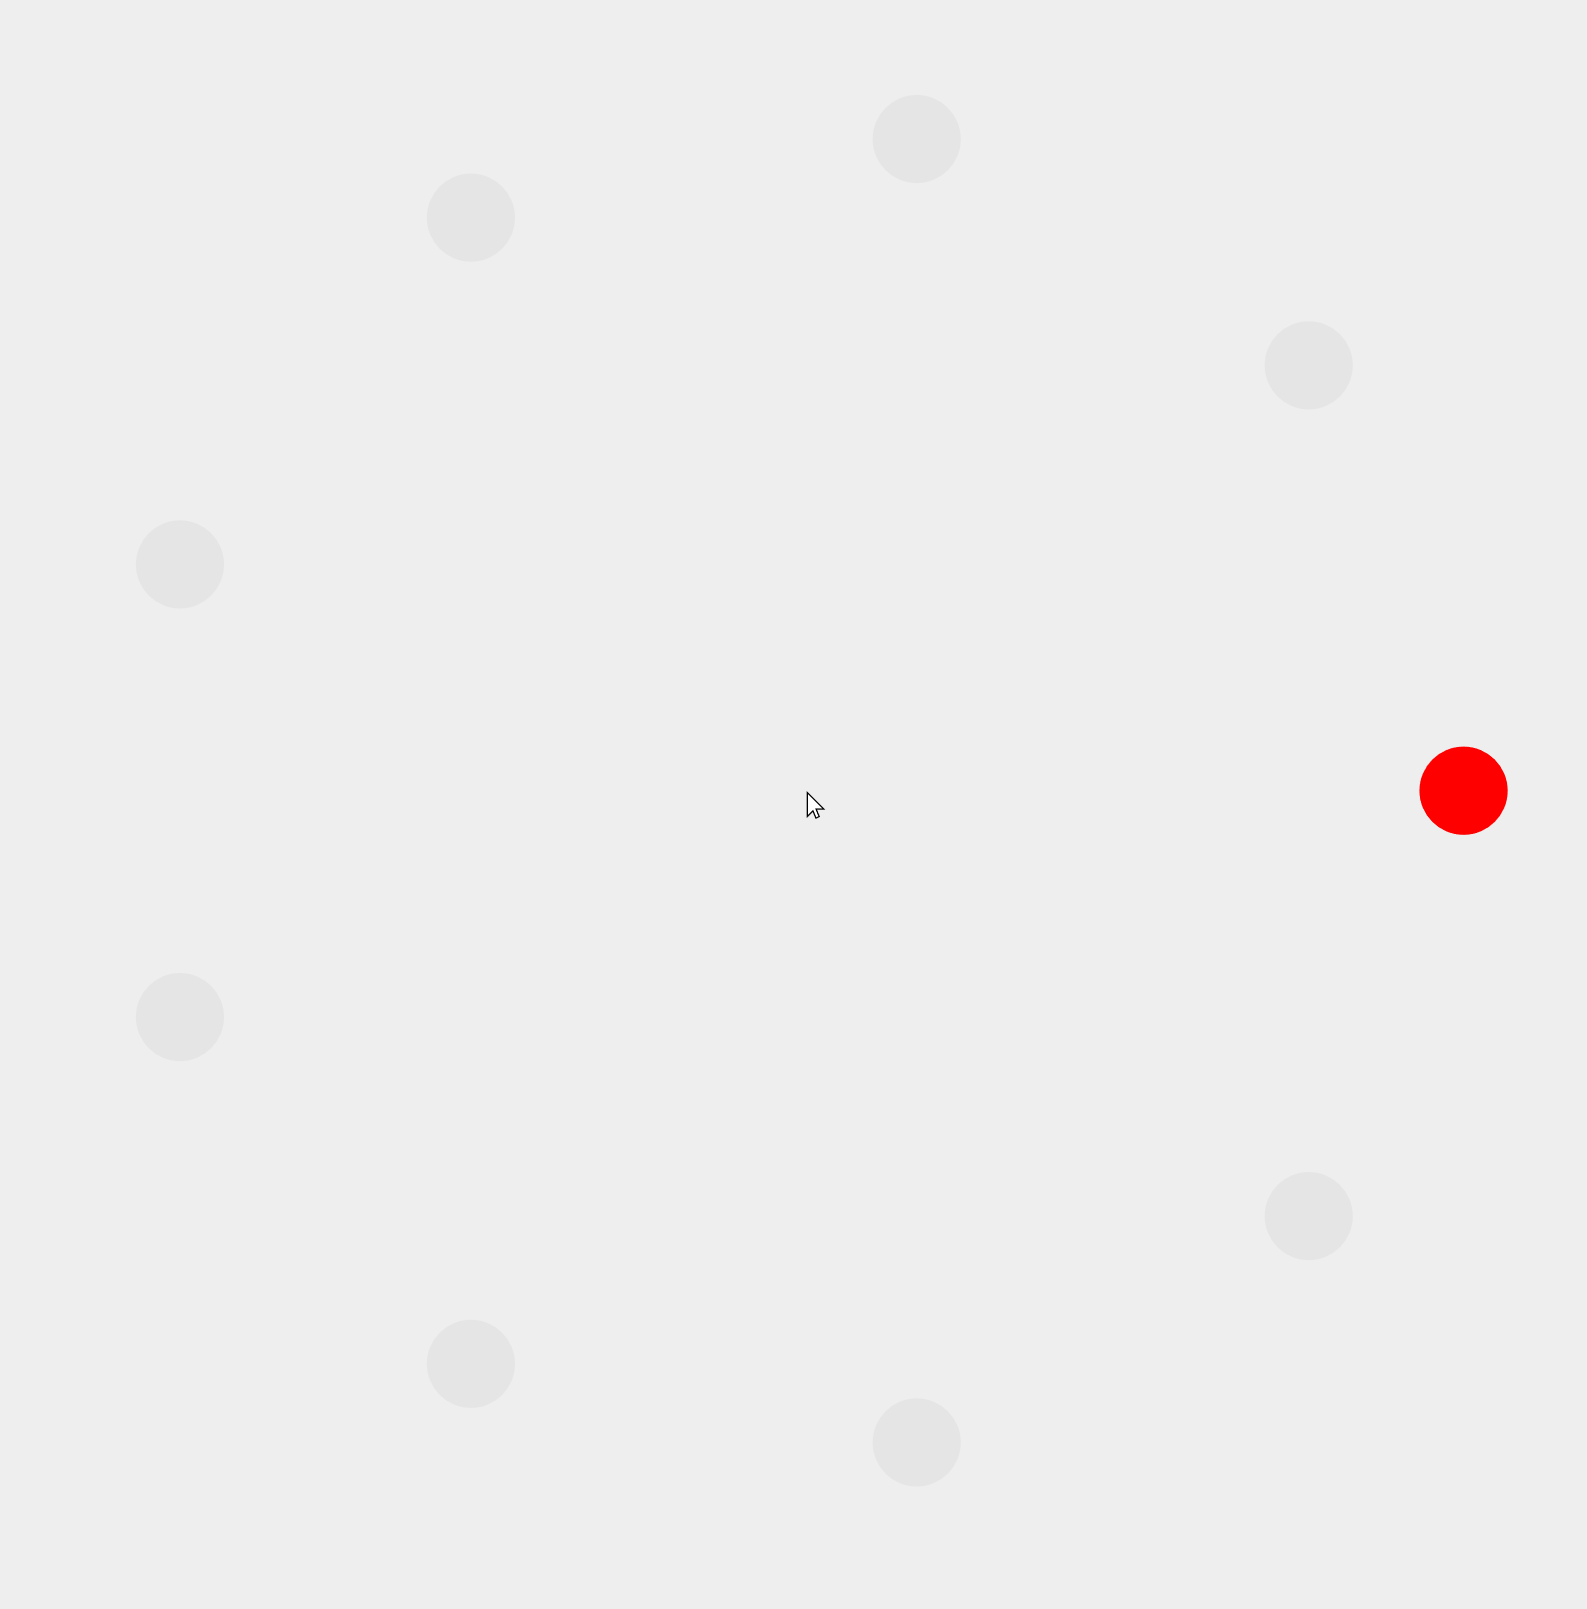
\includegraphics[width=0.9\columnwidth]{Interface}
    \caption{The Fitts' Law interface used by participants, with the target highlighted in red and possible targets in dark gray.}
    \label{fig:interface}
\end{figure}

After completing the calibration phase, participants are trained on each function, {Constant, Acceleration, RubberEdge} with a fixed distance (118mm) and width (7.9mm) of the targets, an example of the interface presented to participants is seen in Figure \ref{fig:interface}

Once training is complete, participants are presented with one of the three transfer functions and are asked to complete the task for all distance and width combinations. After which the combinations are repeated for the other transfer functions, with a 30 second break between each transfer function. The order of the distance and width combinations are randomised for each transfer function and each participant, using the Durstenfeld shuffle algorithm.

After completing the experiment, participants are asked to complete a survey evaluating each transfer function.

\subsection{Interface problems}\label{section:interface_problems}
A major flaw of the experiment was the transmission of data between the laptop and phone. Due to the instability of wireless communications, the pointer would move in a slightly staggered motion, often inducing a noticeable lag, this did affect the observed performance of the participants in the study. A solution to this problem would be changing the communication method to be over USB; however, the development time involved made this solution unfeasible.

\subsection{Participants}
Seven people (3 female, 4 male) participated in the experiment; participants were in the age range of (15 - 25) years, except for one in the age range of (45 - 55) years. Participants were asked the average number of hours spent using a touchpad each day; responses were varied from not using a touchpad at all to greater than 8 hours per day. Operating system use varied between participants, with five using Windows and one for each MacOS and Linux. Preference for existing pointer acceleration on touchpads also varied, four participants, preferred acceleration, one did not, and two either had no preference or did not know what pointer acceleration was.

\subsection{Design}
A within-subjects design was used. The independent variables were Transfer Function (Constant, Acceleration, RubberEdge), target Distance (D$_S$ - 79mm, D$_M$ 118mm, D$_L$ - 157mm) and target Widths (W$_S$ - 11.8mm, W$_M$ - 7.9mm, W$_S$ 3.9mm) The dependent variables measured were the time between selecting targets and the number of clutches performed to select a target.

Each distance and width combination is pre-set with a sequence of nine targets for the user to select. With three different distances and three widths makes nine unique distance and width combinations. This gave seven Fitts' \gls{ID}\cite{MacKenzie1992FittsInteraction}

For the Constant transfer function, a \gls{CD} gain of 2 was used, this was to encourage clutching and was similar to the default system transfer function provided by Windows 10. The acceleration transfer function was the default provided by Windows 10. The transfer function for RubberEdge in the isotonic was set to a \gls{CD} gain of 2. In the elastic zone, the average velocity of the last three data points from the isotonic zone is used as the initial velocity, from then an acceleration multiplier relative to the distance away from the edge of the isotonic and elastic zone is applied. When the participant is stationary in the elastic zone the pointer is updated at a rate of 400Hz, which is equivalent to the update rate of the touchpad of the laptop. A limit is applied on the maximum velocity that can be obtained by the pointer; this is to prevent the pointer running away from the participant and make the behaviour more predictable.

The order of the transfer functions was counterbalanced between participants using the Latin Squares method. This is to avoid any asymmetric skill transfer induced by training. 

The experiment lasted approximately 15 minutes.

The total number of trials conducted are:\\
7 Participants $\times$ 3 Transfer Functions $\times$ 3 Distances $\times$ 3 Widths $\times$ 9 targets\\
$=$ 1701 total trials